\documentclass{article}
\usepackage{cite}
\usepackage{graphicx}
\usepackage{amsmath}
\newcommand\norm[1]{\left\lVert#1\right\rVert}
\DeclareMathOperator*{\argmin}{arg\,min}

\setlength{\parindent}{0cm}
\setlength{\parskip}{0.25cm}

\begin{document}
\author{Max Horowitz-Gelb}
\title{Active Learning For DBSI: DNA Binding Site Identifier }
\maketitle

\section*{Abstract}
DBSI is a structure based method for predicting the positions of protein interaction sites associated with DNA binding \cite{dbsi}. Here I present a method for applying active learning to the training of DBSI. This method optimizes the training of DBSI in a way that considers the batch style form of labelled data collection necessary when creating a training set. This method shows slight improvements in efficiency in comparison to naive methods. 
\section*{Introduction}
For area under an ROC curve, DBSI has been shown to achieve $~88\%$, a high degree of separability. The score was achieved by training DBSI on a set of 263 unique proteins. The model as a result of this training is now accessible to anyone on a public server \cite{dbsi_server}. The quality of this model could be improved further by training with more labelled data. But to collect more data practically we need to address practical issues.
\subsection*{Necessity for Active Learning}
Unlike learning on data generated from sensors or internet activity, aquiring labelled data for DBSI requires considerable time and energy. Experiments must be done to probe each protein for interaction sites.

\textbf{Find out how protein complexes are aquired to emphasize lab work.}

\subsection*{Neccessity for batch style active learning}
Due to the way training data for DBSI is aquired, standard active learning methods are not appropriate. This is because each training point given to DBSI corresponds to one residue in a protein. Therefore each protein that is probed will give hundreds of new training points. Because of this we must query training points in batches as opposed to querying individual residues. This puts us in a unique situation where the batch with the most informative set training points as a whole may be different than the batch containing the one individually most informative training point. To address this issue I use a active learning querying method which scores batches rather than individual points in order to select the next query protein.

     
\section*{Methods}
DBSI uses a support vector machine to classify residues. Such machine learning model has geometric properties that make applying active learning quite intuitive. 

\subsection*{Non Batch-Style Active Learning SVM}
Let us conside a standard binary classifier SVM as DBSI uses.
Then we have a set of $n$ training examples
$
\{(x_1,y_1),...,(x_n, y_n)\} \subset (X \times \{-1,1\})^n
$ where $X$ denotes our input space. 


 as shown in \cite{svm}, our decision function can be described by its training examples,
\[
g(x) = \sum_{i=1}^{n} \alpha_i k( x_i, x)
\]
and classifcation is simply the sign,
\[
	f(x) = sign(g(x))
\]
Where $x_i$ is the set of support vectors,
$x$ is our vector we want to classify, $\alpha_i$ selects our support vectors, and $k$ is our kernel function.

As shown in \cite{active_learning}, if our kernel $k$ satisfies Mercer's condition, then there exists a feature space $F$ and a map $\phi$ from $X$ to $F$, such that $k(x,x') = \langle \phi(x) , \phi(x') \rangle$, and we may rewrite our above equation as
 
\[
f(x) = sign(\langle w_{svm}, \phi(x) \rangle)
\]
\[
w_{svm} = \sum_{i=1}^n \alpha_i \phi(x_i)
\]
where $w_{svm}$ is the normal vector of our hyperplane in feature space. 

If we assume our training data is linearly separable in $F$ then there is exists a non-empty set
\[
V = \{w \in F | y_i \langle w, \phi(x_i) \rangle > 0 \text{ for } i = 1, ...,n \text{ and} \norm{w} = 1
\]
which we call our version space \cite{version_space}.

Now let $Q \in X^m$ be our query pool that our active learner has access to and
$l : X \rightarrow \{-1,1\}$ be a function giving the correct label of an instance of our query pool.

Then at each step our active learner removes one instance $x_{n+1}$ from $Q$ and then adds it to our training set with the result
\[
\{(x_1, y_1),...,(x_n,y_n)\}\cup\{(x_{n+1}, l(x_{n+1})\}
\]


For an efficient learning we want an active learner who most rapidly decays the cardinality of $V$ as it adds individual examples to our training set. As shown in \cite{active_learning} we can guarantee a high decay in $|V|$ by querying the point closest to the hyperplane in feature space. So at each active learning query step we query
\[
x_{n+1} = \argmin_{x' \in Q} g(x')
\]

For active learning in a setting where we query one instance at a time, this works fairly well, but this is not the case in batch style active learning. 

\subsection*{Batch-Style Active Learning}



  






\cite{active_learning}
\section*{Results}
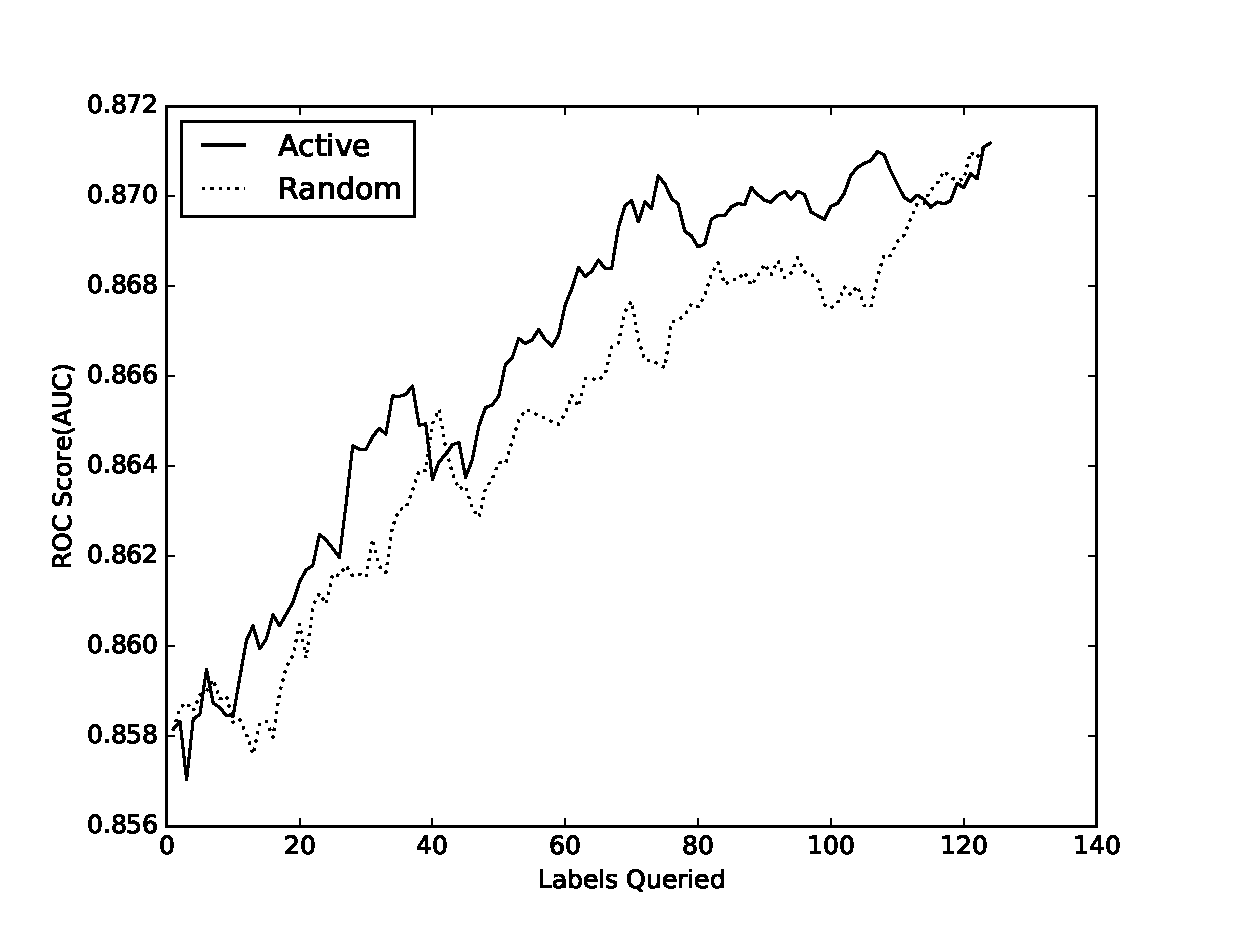
\includegraphics[scale=0.5]{plot}
\section*{Conclusion}

\bibliographystyle{plain}
\bibliography{mybib}{}

\end{document}
